% Options for packages loaded elsewhere
\PassOptionsToPackage{unicode}{hyperref}
\PassOptionsToPackage{hyphens}{url}
%
\documentclass[
]{article}
\usepackage{lmodern}
\usepackage{amssymb,amsmath}
\usepackage{ifxetex,ifluatex}
\ifnum 0\ifxetex 1\fi\ifluatex 1\fi=0 % if pdftex
  \usepackage[T1]{fontenc}
  \usepackage[utf8]{inputenc}
  \usepackage{textcomp} % provide euro and other symbols
\else % if luatex or xetex
  \usepackage{unicode-math}
  \defaultfontfeatures{Scale=MatchLowercase}
  \defaultfontfeatures[\rmfamily]{Ligatures=TeX,Scale=1}
\fi
% Use upquote if available, for straight quotes in verbatim environments
\IfFileExists{upquote.sty}{\usepackage{upquote}}{}
\IfFileExists{microtype.sty}{% use microtype if available
  \usepackage[]{microtype}
  \UseMicrotypeSet[protrusion]{basicmath} % disable protrusion for tt fonts
}{}
\makeatletter
\@ifundefined{KOMAClassName}{% if non-KOMA class
  \IfFileExists{parskip.sty}{%
    \usepackage{parskip}
  }{% else
    \setlength{\parindent}{0pt}
    \setlength{\parskip}{6pt plus 2pt minus 1pt}}
}{% if KOMA class
  \KOMAoptions{parskip=half}}
\makeatother
\usepackage{xcolor}
\IfFileExists{xurl.sty}{\usepackage{xurl}}{} % add URL line breaks if available
\IfFileExists{bookmark.sty}{\usepackage{bookmark}}{\usepackage{hyperref}}
\hypersetup{
  pdftitle={Microsimulation Modeling in R},
  pdfauthor={The DARTH workgroup},
  hidelinks,
  pdfcreator={LaTeX via pandoc}}
\urlstyle{same} % disable monospaced font for URLs
\usepackage[margin=1in]{geometry}
\usepackage{longtable,booktabs}
% Correct order of tables after \paragraph or \subparagraph
\usepackage{etoolbox}
\makeatletter
\patchcmd\longtable{\par}{\if@noskipsec\mbox{}\fi\par}{}{}
\makeatother
% Allow footnotes in longtable head/foot
\IfFileExists{footnotehyper.sty}{\usepackage{footnotehyper}}{\usepackage{footnote}}
\makesavenoteenv{longtable}
\usepackage{graphicx,grffile}
\makeatletter
\def\maxwidth{\ifdim\Gin@nat@width>\linewidth\linewidth\else\Gin@nat@width\fi}
\def\maxheight{\ifdim\Gin@nat@height>\textheight\textheight\else\Gin@nat@height\fi}
\makeatother
% Scale images if necessary, so that they will not overflow the page
% margins by default, and it is still possible to overwrite the defaults
% using explicit options in \includegraphics[width, height, ...]{}
\setkeys{Gin}{width=\maxwidth,height=\maxheight,keepaspectratio}
% Set default figure placement to htbp
\makeatletter
\def\fps@figure{htbp}
\makeatother
\setlength{\emergencystretch}{3em} % prevent overfull lines
\providecommand{\tightlist}{%
  \setlength{\itemsep}{0pt}\setlength{\parskip}{0pt}}
\setcounter{secnumdepth}{-\maxdimen} % remove section numbering

\title{Microsimulation Modeling in R}
\usepackage{etoolbox}
\makeatletter
\providecommand{\subtitle}[1]{% add subtitle to \maketitle
  \apptocmd{\@title}{\par {\large #1 \par}}{}{}
}
\makeatother
\subtitle{Exercises -- Microsimulation models}
\author{The DARTH workgroup}
\date{}

\begin{document}
\maketitle

Developed by the Decision Analysis in R for Technologies in Health
(DARTH) workgroup:

Fernando Alarid-Escudero, PhD (1)

Eva A. Enns, MS, PhD (2)

M.G. Myriam Hunink, MD, PhD (3,4)

Hawre J. Jalal, MD, PhD (5)

Eline M. Krijkamp, MSc (3)

Petros Pechlivanoglou, PhD (6,7)

Alan Yang, MSc (7)

In collaboration of:

\begin{enumerate}
\def\labelenumi{\arabic{enumi}.}
\tightlist
\item
  Drug Policy Program, Center for Research and Teaching in Economics
  (CIDE) - CONACyT, Aguascalientes, Mexico
\item
  University of Minnesota School of Public Health, Minneapolis, MN, USA
\item
  Erasmus MC, Rotterdam, The Netherlands
\item
  Harvard T.H. Chan School of Public Health, Boston, USA
\item
  University of Pittsburgh Graduate School of Public Health, Pittsburgh,
  PA, USA
\item
  University of Toronto, Toronto ON, Canada
\item
  The Hospital for Sick Children, Toronto ON, Canada
\end{enumerate}

Please cite our publications when using this code:

\begin{itemize}
\item
  Jalal H, Pechlivanoglou P, Krijkamp E, Alarid-Escudero F, Enns E,
  Hunink MG. An Overview of R in Health Decision Sciences. Med Decis
  Making. 2017; 37(3): 735-746.
  \url{https://journals.sagepub.com/doi/abs/10.1177/0272989X16686559}
\item
  Krijkamp EM, Alarid-Escudero F, Enns EA, Jalal HJ, Hunink MGM,
  Pechlivanoglou P. Microsimulation modeling for health decision
  sciences using R: A tutorial. Med Decis Making. 2018;38(3):400--22.
  \url{https://journals.sagepub.com/doi/abs/10.1177/0272989X18754513}
\item
  Krijkamp EM, Alarid-Escudero F, Enns E, Pechlivanoglou P, Hunink MM,
  Jalal H. A Multidimensional Array Representation of State-Transition
  Model Dynamics. Med Decis Making. 2020 Online first.
  \url{https://doi.org/10.1177/0272989X19893973}
\end{itemize}

Copyright 2017, THE HOSPITAL FOR SICK CHILDREN AND THE COLLABORATING
INSTITUTIONS. All rights reserved in Canada, the United States and
worldwide. Copyright, trademarks, trade names and any and all associated
intellectual property are exclusively owned by THE HOSPITAL FOR Sick
CHILDREN and the collaborating institutions. These materials may be
used, reproduced, modified, distributed and adapted with proper
attribution.

\hypertarget{exercise-i-a-microsimulation-model-the-sick-sicker-model}{%
\section{Exercise I: A Microsimulation model -- The Sick-Sicker
model}\label{exercise-i-a-microsimulation-model-the-sick-sicker-model}}

In this exercise, we will model a hypothetical disease using an
individual-based state-transition model, or what we often call a
microsimulation model, called the ``Sick-Sicker'' model. This model has
four health states (Figure 1): Healthy (H); two disease states, Sick
(S1) and Sicker (S2); and Dead (D).

Advantages of using a microsimulation implementation is the ability to
incorporate variation in the baseline characteristics for every
individual and to keep track of state-residence. To illustrate this, we
assume that individual mortality rates depend on baseline
characteristics as well as time spend in the sick health state.

After you have successfully implemented the Sick-Sicker model, you can
expand the model to include the possibility of treatment and evaluate
whether it is cost-effective given a willingness to pay of \$20,000.
This hypothetical treatment improves the quality of life for those in
the Sick (S1) state but not for those in the Sicker (S2) state. However,
it is not possible to distinguish between individuals in the Sick state
from those in the Sicker state, so under a treatment strategy,
individuals in both sick states must be treated (and incur the costs of
treatment), while only those in the sick state benefit from it.

In summary, the model assumes the following:

\begin{enumerate}
\def\labelenumi{\roman{enumi})}
\item
  The mortality rates depend on age
\item
  Probability of dying when sick depends on state-residence in the Sick
  (S1) state.
\item
  The improvement on quality of life by the treatment varies across
  individuals through a characteristic that acts as a treatment effect
  modifier.
\end{enumerate}

All model parameter values and \texttt{R} variable names are presented
in Table 1.

\hypertarget{tasks}{%
\subsection{Tasks}\label{tasks}}

There are quite some steps you need to take in order to create a
microsimulation reflecting this case. Start by download all the
materials as a folder or collect all the files in one folder. If there
is an R projects in the folder, a file ending on \texttt{.Rproj}, double
click on this file to open an Rstudio environoment. Working from a
Rproject avoid struggles with working directories.

\begin{enumerate}
\def\labelenumi{\arabic{enumi}.}
\item
  Open the file
  \texttt{microsim\_Sick-Sicker\_time\_full\_template.Rmd}. This is a
  template to load the data for the time dependency and the necessary
  data. Start making the functions \texttt{Probs()}, \texttt{Costs()}
  and \texttt{Effs()}.
\item
  Build your microsimulation model (function). Then, simulate a
  population of 100,000 individuals and plot the resulting distributions
  of remaining lifetime costs and QALYs. Please be reminded that the
  probabilities of transitioning from one state to the other (except to
  the Dead state) are conditional on staying alive.
\item
  Expand your microsimulation model to include the possibility of the
  hypothetical treatment for the disease in the Sick-Sicker model (and
  its impact on costs and quality of life). Remember treatment is given
  to both individuals in Sick and Sicker but only improved the quality
  of life of those in Sick. Create a new variable within the model
  function that can be used to turn treatment on and off in the model.
\item
  Simulate a population of 100,000 individuals under a treatment
  strategy where anyone who is sick (in the Sick or Sicker states)
  receives treatment. Plot the resulting distributions of remaining
  lifetime costs and QALYs.
\item
  Calculate the incremental cost-effectiveness ratio (ICER) of treatment
  compared to no treatment (see code template).
\end{enumerate}

\newpage

\textbf{Table 1: Input parameters for the time dependent Sick-Sicker
Microsimulation }

\begin{longtable}[]{@{}llc@{}}
\toprule
\begin{minipage}[b]{0.51\columnwidth}\raggedright
\textbf{Parameter}\strut
\end{minipage} & \begin{minipage}[b]{0.19\columnwidth}\raggedright
\textbf{R name}\strut
\end{minipage} & \begin{minipage}[b]{0.21\columnwidth}\centering
\textbf{Value}\strut
\end{minipage}\tabularnewline
\midrule
\endhead
\begin{minipage}[t]{0.51\columnwidth}\raggedright
Time horizon\strut
\end{minipage} & \begin{minipage}[t]{0.19\columnwidth}\raggedright
\texttt{n\_t}\strut
\end{minipage} & \begin{minipage}[t]{0.21\columnwidth}\centering
30 years\strut
\end{minipage}\tabularnewline
\begin{minipage}[t]{0.51\columnwidth}\raggedright
Cycle length\strut
\end{minipage} & \begin{minipage}[t]{0.19\columnwidth}\raggedright
\strut
\end{minipage} & \begin{minipage}[t]{0.21\columnwidth}\centering
1 year\strut
\end{minipage}\tabularnewline
\begin{minipage}[t]{0.51\columnwidth}\raggedright
Names of simulated individuals\strut
\end{minipage} & \begin{minipage}[t]{0.19\columnwidth}\raggedright
\texttt{n\_i}\strut
\end{minipage} & \begin{minipage}[t]{0.21\columnwidth}\centering
1000\strut
\end{minipage}\tabularnewline
\begin{minipage}[t]{0.51\columnwidth}\raggedright
Names of health states\strut
\end{minipage} & \begin{minipage}[t]{0.19\columnwidth}\raggedright
\texttt{v\_n}\strut
\end{minipage} & \begin{minipage}[t]{0.21\columnwidth}\centering
H, S1, S2, D\strut
\end{minipage}\tabularnewline
\begin{minipage}[t]{0.51\columnwidth}\raggedright
Annual discount rate (costs/QALYs)\strut
\end{minipage} & \begin{minipage}[t]{0.19\columnwidth}\raggedright
\texttt{d\_e} \texttt{d\_c}\strut
\end{minipage} & \begin{minipage}[t]{0.21\columnwidth}\centering
3\%\strut
\end{minipage}\tabularnewline
\begin{minipage}[t]{0.51\columnwidth}\raggedright
Population characteristics\strut
\end{minipage} & \begin{minipage}[t]{0.19\columnwidth}\raggedright
\strut
\end{minipage} & \begin{minipage}[t]{0.21\columnwidth}\centering
\strut
\end{minipage}\tabularnewline
\begin{minipage}[t]{0.51\columnwidth}\raggedright
- Age distribution\strut
\end{minipage} & \begin{minipage}[t]{0.19\columnwidth}\raggedright
--\strut
\end{minipage} & \begin{minipage}[t]{0.21\columnwidth}\centering
Range:25-55 distributed as in
\texttt{MyPopulation-AgeDistribution.csv}\strut
\end{minipage}\tabularnewline
\begin{minipage}[t]{0.51\columnwidth}\raggedright
Annual transition probabilities conditional on survival\strut
\end{minipage} & \begin{minipage}[t]{0.19\columnwidth}\raggedright
\strut
\end{minipage} & \begin{minipage}[t]{0.21\columnwidth}\centering
\strut
\end{minipage}\tabularnewline
\begin{minipage}[t]{0.51\columnwidth}\raggedright
- Disease onset (H to S1)\strut
\end{minipage} & \begin{minipage}[t]{0.19\columnwidth}\raggedright
\texttt{p\_HS1}\strut
\end{minipage} & \begin{minipage}[t]{0.21\columnwidth}\centering
0.15\strut
\end{minipage}\tabularnewline
\begin{minipage}[t]{0.51\columnwidth}\raggedright
- Recovery (S1 to H)\strut
\end{minipage} & \begin{minipage}[t]{0.19\columnwidth}\raggedright
\texttt{p\_S1H}\strut
\end{minipage} & \begin{minipage}[t]{0.21\columnwidth}\centering
0.5\strut
\end{minipage}\tabularnewline
\begin{minipage}[t]{0.51\columnwidth}\raggedright
- Disease progression (S1 to S2)\strut
\end{minipage} & \begin{minipage}[t]{0.19\columnwidth}\raggedright
\texttt{p\_S1S2}\strut
\end{minipage} & \begin{minipage}[t]{0.21\columnwidth}\centering
0.105\strut
\end{minipage}\tabularnewline
\begin{minipage}[t]{0.51\columnwidth}\raggedright
Annual mortality\strut
\end{minipage} & \begin{minipage}[t]{0.19\columnwidth}\raggedright
\strut
\end{minipage} & \begin{minipage}[t]{0.21\columnwidth}\centering
\strut
\end{minipage}\tabularnewline
\begin{minipage}[t]{0.51\columnwidth}\raggedright
- All-cause mortality (H to D)\strut
\end{minipage} & \begin{minipage}[t]{0.19\columnwidth}\raggedright
\texttt{p\_HD}\strut
\end{minipage} & \begin{minipage}[t]{0.21\columnwidth}\centering
Human Mortality Database (\texttt{mortProb\_age.csv}): age dependent
from 2015\strut
\end{minipage}\tabularnewline
\begin{minipage}[t]{0.51\columnwidth}\raggedright
- Probability of death is S1 (S1 to D)\strut
\end{minipage} & \begin{minipage}[t]{0.19\columnwidth}\raggedright
\texttt{p\_S1D}\strut
\end{minipage} & \begin{minipage}[t]{0.21\columnwidth}\centering
*(in template)\strut
\end{minipage}\tabularnewline
\begin{minipage}[t]{0.51\columnwidth}\raggedright
- Probability of death in S2 (S2 to D)\strut
\end{minipage} & \begin{minipage}[t]{0.19\columnwidth}\raggedright
\texttt{p\_S2D}\strut
\end{minipage} & \begin{minipage}[t]{0.21\columnwidth}\centering
0.048\strut
\end{minipage}\tabularnewline
\begin{minipage}[t]{0.51\columnwidth}\raggedright
Annual costs\strut
\end{minipage} & \begin{minipage}[t]{0.19\columnwidth}\raggedright
\strut
\end{minipage} & \begin{minipage}[t]{0.21\columnwidth}\centering
\strut
\end{minipage}\tabularnewline
\begin{minipage}[t]{0.51\columnwidth}\raggedright
- Healthy individuals\strut
\end{minipage} & \begin{minipage}[t]{0.19\columnwidth}\raggedright
\texttt{c\_H}\strut
\end{minipage} & \begin{minipage}[t]{0.21\columnwidth}\centering
\$2,000\strut
\end{minipage}\tabularnewline
\begin{minipage}[t]{0.51\columnwidth}\raggedright
- Sick individuals in S1\strut
\end{minipage} & \begin{minipage}[t]{0.19\columnwidth}\raggedright
\texttt{c\_S1}\strut
\end{minipage} & \begin{minipage}[t]{0.21\columnwidth}\centering
\$4,000\strut
\end{minipage}\tabularnewline
\begin{minipage}[t]{0.51\columnwidth}\raggedright
- Sick individuals in S2\strut
\end{minipage} & \begin{minipage}[t]{0.19\columnwidth}\raggedright
\texttt{c\_S2}\strut
\end{minipage} & \begin{minipage}[t]{0.21\columnwidth}\centering
\$15,000\strut
\end{minipage}\tabularnewline
\begin{minipage}[t]{0.51\columnwidth}\raggedright
- Dead individuals\strut
\end{minipage} & \begin{minipage}[t]{0.19\columnwidth}\raggedright
\texttt{c\_D}\strut
\end{minipage} & \begin{minipage}[t]{0.21\columnwidth}\centering
\$0\strut
\end{minipage}\tabularnewline
\begin{minipage}[t]{0.51\columnwidth}\raggedright
- Additional costs of sick individuals treated in S1 or S2\strut
\end{minipage} & \begin{minipage}[t]{0.19\columnwidth}\raggedright
\texttt{c\_trt}\strut
\end{minipage} & \begin{minipage}[t]{0.21\columnwidth}\centering
\$12,000\strut
\end{minipage}\tabularnewline
\begin{minipage}[t]{0.51\columnwidth}\raggedright
Utility weights\strut
\end{minipage} & \begin{minipage}[t]{0.19\columnwidth}\raggedright
\strut
\end{minipage} & \begin{minipage}[t]{0.21\columnwidth}\centering
\strut
\end{minipage}\tabularnewline
\begin{minipage}[t]{0.51\columnwidth}\raggedright
- Healthy individuals\strut
\end{minipage} & \begin{minipage}[t]{0.19\columnwidth}\raggedright
\texttt{u\_H}\strut
\end{minipage} & \begin{minipage}[t]{0.21\columnwidth}\centering
1.00\strut
\end{minipage}\tabularnewline
\begin{minipage}[t]{0.51\columnwidth}\raggedright
- Sick individuals in S1\strut
\end{minipage} & \begin{minipage}[t]{0.19\columnwidth}\raggedright
\texttt{u\_S1}\strut
\end{minipage} & \begin{minipage}[t]{0.21\columnwidth}\centering
0.75\strut
\end{minipage}\tabularnewline
\begin{minipage}[t]{0.51\columnwidth}\raggedright
- Sick individuals in S2\strut
\end{minipage} & \begin{minipage}[t]{0.19\columnwidth}\raggedright
\texttt{u\_S2}\strut
\end{minipage} & \begin{minipage}[t]{0.21\columnwidth}\centering
0.50\strut
\end{minipage}\tabularnewline
\begin{minipage}[t]{0.51\columnwidth}\raggedright
- Dead individuals\strut
\end{minipage} & \begin{minipage}[t]{0.19\columnwidth}\raggedright
\texttt{u\_D}\strut
\end{minipage} & \begin{minipage}[t]{0.21\columnwidth}\centering
0.00\strut
\end{minipage}\tabularnewline
\begin{minipage}[t]{0.51\columnwidth}\raggedright
Intervention effect\strut
\end{minipage} & \begin{minipage}[t]{0.19\columnwidth}\raggedright
\strut
\end{minipage} & \begin{minipage}[t]{0.21\columnwidth}\centering
\strut
\end{minipage}\tabularnewline
\begin{minipage}[t]{0.51\columnwidth}\raggedright
- Utility for treated individuals in S1\strut
\end{minipage} & \begin{minipage}[t]{0.19\columnwidth}\raggedright
\texttt{u\_trt}\strut
\end{minipage} & \begin{minipage}[t]{0.21\columnwidth}\centering
0.95\strut
\end{minipage}\tabularnewline
\begin{minipage}[t]{0.51\columnwidth}\raggedright
Time varying extension of Sick-Sicker model\strut
\end{minipage} & \begin{minipage}[t]{0.19\columnwidth}\raggedright
\strut
\end{minipage} & \begin{minipage}[t]{0.21\columnwidth}\centering
\strut
\end{minipage}\tabularnewline
\begin{minipage}[t]{0.51\columnwidth}\raggedright
- Treatment effect modifier at baseline\strut
\end{minipage} & \begin{minipage}[t]{0.19\columnwidth}\raggedright
\texttt{v\_x}\strut
\end{minipage} & \begin{minipage}[t]{0.21\columnwidth}\centering
Uniform(0.95, 1.05)\strut
\end{minipage}\tabularnewline
\bottomrule
\end{longtable}

\begin{figure}

{\centering 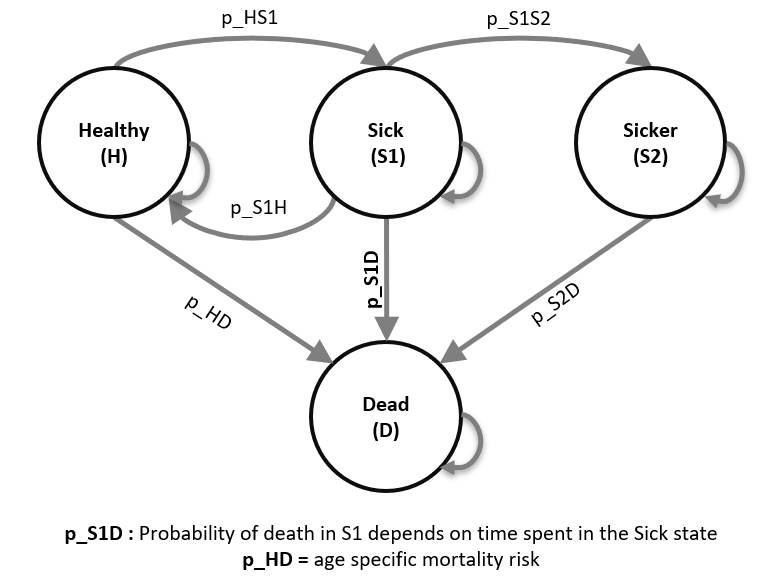
\includegraphics[width=1\linewidth]{sick_sicker_diagram_time} 

}

\caption{Schematic representation of the Sick-Sicker model}\label{fig:unnamed-chunk-1}
\end{figure}

\newpage

\hypertarget{exercise-ii-probabilistic-sensitivity-analysis-of-the-sick-sicker-microsimulation-model}{%
\section{Exercise II: Probabilistic sensitivity analysis of the
Sick-Sicker microsimulation
model}\label{exercise-ii-probabilistic-sensitivity-analysis-of-the-sick-sicker-microsimulation-model}}

This exercise continues based on the microsimulation model of the
Sick-Sicker model from Exercise I. For the Sick-Sicker model you just
created, you will develop a probabilistic sensitivity analysis (PSA)
with 1000 simulations \texttt{(n\_sim)}. The Table describes the
distributions for the variables you used in the previous exercise.

\textbf{Table II: Input parameters for probabilistic analysis}

\begin{longtable}[]{@{}lrr@{}}
\toprule
\begin{minipage}[b]{0.32\columnwidth}\raggedright
\textbf{Parameter}\strut
\end{minipage} & \begin{minipage}[b]{0.17\columnwidth}\raggedleft
\textbf{Distribution}\strut
\end{minipage} & \begin{minipage}[b]{0.42\columnwidth}\raggedleft
\textbf{Distribution values}\strut
\end{minipage}\tabularnewline
\midrule
\endhead
\begin{minipage}[t]{0.32\columnwidth}\raggedright
Number of simulation\strut
\end{minipage} & \begin{minipage}[t]{0.17\columnwidth}\raggedleft
\texttt{n\_sim}\strut
\end{minipage} & \begin{minipage}[t]{0.42\columnwidth}\raggedleft
1000\strut
\end{minipage}\tabularnewline
\begin{minipage}[t]{0.32\columnwidth}\raggedright
Annual transition probabilities\strut
\end{minipage} & \begin{minipage}[t]{0.17\columnwidth}\raggedleft
\strut
\end{minipage} & \begin{minipage}[t]{0.42\columnwidth}\raggedleft
\strut
\end{minipage}\tabularnewline
\begin{minipage}[t]{0.32\columnwidth}\raggedright
- Disease onset (H to S1)\strut
\end{minipage} & \begin{minipage}[t]{0.17\columnwidth}\raggedleft
Beta\strut
\end{minipage} & \begin{minipage}[t]{0.42\columnwidth}\raggedleft
\(\alpha=30, \ \beta=170\)\strut
\end{minipage}\tabularnewline
\begin{minipage}[t]{0.32\columnwidth}\raggedright
- Recovery (S1 to H)\strut
\end{minipage} & \begin{minipage}[t]{0.17\columnwidth}\raggedleft
Beta\strut
\end{minipage} & \begin{minipage}[t]{0.42\columnwidth}\raggedleft
\(\alpha=60, \ \beta=60\)\strut
\end{minipage}\tabularnewline
\begin{minipage}[t]{0.32\columnwidth}\raggedright
- Disease progression (S1 to S2)\strut
\end{minipage} & \begin{minipage}[t]{0.17\columnwidth}\raggedleft
Beta\strut
\end{minipage} & \begin{minipage}[t]{0.42\columnwidth}\raggedleft
\(\alpha=84, \ \beta=716\)\strut
\end{minipage}\tabularnewline
\begin{minipage}[t]{0.32\columnwidth}\raggedright
- Probability of death in S2 (S2 to D)\strut
\end{minipage} & \begin{minipage}[t]{0.17\columnwidth}\raggedleft
Beta\strut
\end{minipage} & \begin{minipage}[t]{0.42\columnwidth}\raggedleft
\(\alpha=22, \ \beta=434\)\strut
\end{minipage}\tabularnewline
\begin{minipage}[t]{0.32\columnwidth}\raggedright
Annual costs\strut
\end{minipage} & \begin{minipage}[t]{0.17\columnwidth}\raggedleft
\strut
\end{minipage} & \begin{minipage}[t]{0.42\columnwidth}\raggedleft
\strut
\end{minipage}\tabularnewline
\begin{minipage}[t]{0.32\columnwidth}\raggedright
- Healthy individuals\strut
\end{minipage} & \begin{minipage}[t]{0.17\columnwidth}\raggedleft
Gamma\strut
\end{minipage} & \begin{minipage}[t]{0.42\columnwidth}\raggedleft
shape = 100.0, scale = 20.0\strut
\end{minipage}\tabularnewline
\begin{minipage}[t]{0.32\columnwidth}\raggedright
- Sick individuals in S1\strut
\end{minipage} & \begin{minipage}[t]{0.17\columnwidth}\raggedleft
Gamma\strut
\end{minipage} & \begin{minipage}[t]{0.42\columnwidth}\raggedleft
shape = 177.8, scale = 22.5\strut
\end{minipage}\tabularnewline
\begin{minipage}[t]{0.32\columnwidth}\raggedright
- Sick individuals in S2\strut
\end{minipage} & \begin{minipage}[t]{0.17\columnwidth}\raggedleft
Gamma\strut
\end{minipage} & \begin{minipage}[t]{0.42\columnwidth}\raggedleft
shape = 225.0, scale = 66.7\strut
\end{minipage}\tabularnewline
\begin{minipage}[t]{0.32\columnwidth}\raggedright
- Additional costs of sick individuals treated in S1 or S2\strut
\end{minipage} & \begin{minipage}[t]{0.17\columnwidth}\raggedleft
Gamma\strut
\end{minipage} & \begin{minipage}[t]{0.42\columnwidth}\raggedleft
shape = 73.5, scale = 163.3\strut
\end{minipage}\tabularnewline
\begin{minipage}[t]{0.32\columnwidth}\raggedright
Utility weights\strut
\end{minipage} & \begin{minipage}[t]{0.17\columnwidth}\raggedleft
\strut
\end{minipage} & \begin{minipage}[t]{0.42\columnwidth}\raggedleft
\strut
\end{minipage}\tabularnewline
\begin{minipage}[t]{0.32\columnwidth}\raggedright
- Healthy individuals\strut
\end{minipage} & \begin{minipage}[t]{0.17\columnwidth}\raggedleft
Beta\strut
\end{minipage} & \begin{minipage}[t]{0.42\columnwidth}\raggedleft
\(\alpha = 200, \ \beta = 3\)\strut
\end{minipage}\tabularnewline
\begin{minipage}[t]{0.32\columnwidth}\raggedright
- Sick individuals in S1\strut
\end{minipage} & \begin{minipage}[t]{0.17\columnwidth}\raggedleft
Beta\strut
\end{minipage} & \begin{minipage}[t]{0.42\columnwidth}\raggedleft
\(\alpha = 130, \ \beta = 45\)\strut
\end{minipage}\tabularnewline
\begin{minipage}[t]{0.32\columnwidth}\raggedright
- Sick individuals in S2\strut
\end{minipage} & \begin{minipage}[t]{0.17\columnwidth}\raggedleft
Beta\strut
\end{minipage} & \begin{minipage}[t]{0.42\columnwidth}\raggedleft
\(\alpha = 230, \ \beta = 230\)\strut
\end{minipage}\tabularnewline
\begin{minipage}[t]{0.32\columnwidth}\raggedright
Intervention effect\strut
\end{minipage} & \begin{minipage}[t]{0.17\columnwidth}\raggedleft
\strut
\end{minipage} & \begin{minipage}[t]{0.42\columnwidth}\raggedleft
\strut
\end{minipage}\tabularnewline
\begin{minipage}[t]{0.32\columnwidth}\raggedright
- Utility for treated individuals in S1\strut
\end{minipage} & \begin{minipage}[t]{0.17\columnwidth}\raggedleft
Beta\strut
\end{minipage} & \begin{minipage}[t]{0.42\columnwidth}\raggedleft
\(\alpha = 300, \ \beta = 15\)\strut
\end{minipage}\tabularnewline
\bottomrule
\end{longtable}

\hypertarget{tasks-1}{%
\subsection{Tasks}\label{tasks-1}}

The tasks below help you to develop a probabilistic sensitivity analysis
(PSA). Please note that these tasks are very similar to what was
demonstrated in the 3-state microsimulation model example and that you
can use the Sick-Sicker model you already created.

\begin{enumerate}
\def\labelenumi{\arabic{enumi}.}
\setcounter{enumi}{5}
\item
  Create the \texttt{calculate\_ce\_out} \texttt{R} function of the
  Sick-Sicker microsimulation model and store in a separate \texttt{R}
  file \texttt{Function\_Microsim\_Sick-Sicker\_time.R}.
\item
  Create a function called \texttt{gen\_psa} to sample values for the
  uncertain parameters using the appropriate distributions.
\item
  Open the file \texttt{microsim\_Sick-Sicker\_time\_template.R} and
  conduct a probabilistic Cost-Effectiveness analysis of treatment vs
  no-treatment.
\item
  Create histograms of model inputs.
\item
  Create a cost-effectiveness plane to present discounted costs and
  QALYs.
\end{enumerate}

Extra 1: The solutions will provide you code to create a
cost-effectiveness acceptability curves (CEAC) and frontier (CEAF) for
the treatment comparison assuming WTP thresholds of \(\$0\) to
\(\$300,000\).

Extra 2: The solutions will provide code to calculate the expected value
of perfect information (EVPI)

\end{document}
